Como explanado anteriormente, o motor de passo híbrido congrega características do motor de passo de ímã permanente e o motor de passo de relutância variável. Para entender como o motor de passo híbrido funciona, primeiramente irá ser mostrado brevemente o princípio de funcionamento destes dois outros tipos de motores de passo ora citados, bem como o que são motores de passo, por fim será explicado o funcionamento do motor de passo híbrido em função como um motor aperfeiçoado dos outros dois motores de passo, a fim da explicação se tornar mais familiarizada para o leitor.  

	\subsection{Motor de passo genérico}
	São máquinas elétricas que consistem em um estator com enrolamentos de excitação e um rotor magnético com saliências. Neles o conjugado é produzido pela tendência do rotor a se alinhar com a onda de fluxo produzida pelo estator, de modo a maximizar os fluxos concatenados que resultam da aplicação de uma dada corrente no estator. No motor de passo as fases dos enrolamentos do estator são excitadas sequencialmente, fazendo o rotor girar na forma de uma sequência de passos, com ângulos definidos a cada passo, devido à tendência de alinhamento do rotor com a onda de fluxo do estator. \cite{Fitz} As principais características dos motores de passo são \cite{MoonsHSM}:
	
	\begin{itemize}
		\item \textbf{Inexistência de escovas:} não necessitam de escovas, reduzindo a maioria das falhas comumente encontradas nos outros motores elétricos, como faiscamento e perdas ôhmicas no rotor e escovas.
		\item \textbf{Independência da carga:} giram com uma dada velocidade independentemente da carga, desde que tal carga não exceda as característica de torque do motor.
		\item \textbf{Menos sensores} se movem com incrementos quantificáveis, desde que com torque especificado, podendo ter conhecimento da posição do eixo.
		\item \textbf{Posição de repouso:} é possível manter o eixo estacionário, desde que seu torque seja respeitado. 
	\end{itemize}
	
	\subsection{Características construtivas gerais do HSM}
	
	Conforme citado anteriormente, o HSM contêm características importantes do VRM e do PMM, o que justifica a denominação 'híbrido'. O estator de um HSM é exatamente um estator do PMM, enquanto que o rotor de um HSM é um rotor do VRM magnetizado.
	
	Como forma de visualizar melhor as duas partes do motor, a Fig. \ref{HSMreal} apresenta o estator e o rotor de um HSM genérico aberto. As especificações deste motor são bem semelhantes ao motor apresentado na Fig. \ref{HSMgrafico}.
	
	\begin{figure}[!h]
		\centering
		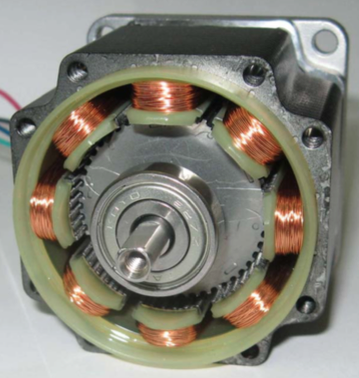
\includegraphics[scale=.45]{Images/hsmreal1.png}
		\caption{Principais partes de um HSM genérico - Visão geral \cite{ieeeRusso}}
		\label{HSMreal}
	\end{figure} 
	
	O estator de um motor de passo híbrido é composto por um dado número de polos magnéticos relacionados com o número de enrolamentos nele, exatamente como em um PMM. Essa característica é herdada dos motores de imã permanente. No PMM, admite-se que para melhorar a resolução de passo, basta adicionar mais enrolamentos ou adicionar mais pares de polos no rotor, através do campo magnético produzido nos enrolamentos deste estator. 
	
	O rotor de um motor de passo híbrido é cuidadosamente seccionado, criando pequenas lacunas chamadas dentes (\textit{teeth}) para gerar uma compensação (\textit{offset}) com relação ao estator para o rotor executar a rotação. É importante citar que o rotor de um HSM é magnetizado, diferentemente do rotor de um VRM.
	
	\begin{figure}[!h]
		\centering
		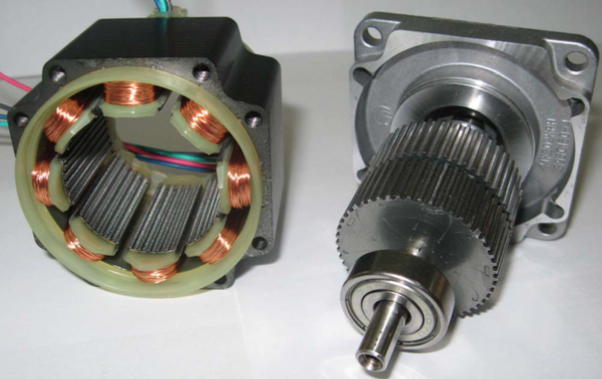
\includegraphics[scale=.4]{Images/hsmreal2.png}
		\caption{Estator (à esquerda) e rotor (à direita) de um HSM genérico \cite{ieeeRusso}}
		\label{HSMestatorrotor}
	\end{figure} 
	
	Verifica-se pela Fig. \ref{HSMestatorrotor} que o estator também é seccionado com alguns dentes. A razão do estator também possuir esses dentes é com o propósito de fazer o motor operar, o que será explanado a seguir.
	
	\subsection{Princípio de funcionamento básico de um motor de passo híbrido}
	
	Conforme pode ser visto na Fig. \ref{HSMestatorrotor}, o rotor de um HSM é seccionado em polos magnéticos que chamaremos de seção sul e seção norte, também denominados \textit{rotor cups}. Essa separação pode ser vista na Fig. \ref{rotorsec}.
	
	\begin{figure}[!h]
		\centering 
		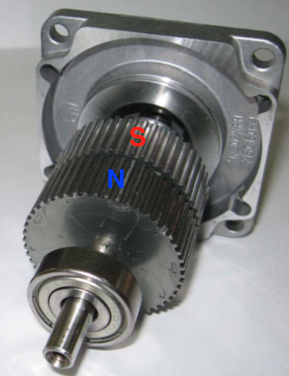
\includegraphics[scale=0.45]{images/hsm_operation/hsmrotorreal}
		\caption{Rotor seccionado em seção sul (S) e seção norte (N) \cite{ieeeRusso}}
		\label{rotorsec}
	\end{figure}
	
	Como apresentado anteriomente e melhor explanado na seção de Características Construtivas do HSM, o rotor é feito com material ferromagnético. De maneira simplificada, apresenta-se o rotor apresentado na Fig. \ref{rotorsec} da seguinte maneira, conforme a Fig. \ref{rotor1}.
	
	\begin{figure}[!h]
		\centering 
		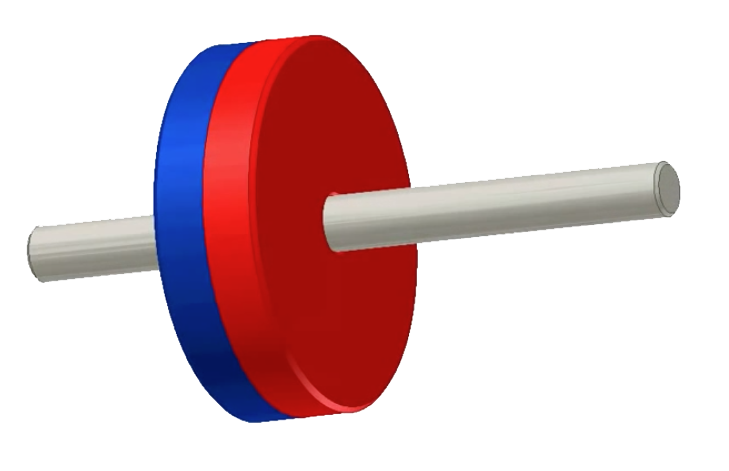
\includegraphics[scale=0.2]{images/hsm_operation/rotormag1}
		\caption{Material ferromagnético do rotor simplificado de um HSM (Sem dentes)}
		\label{rotor1}
	\end{figure}
	
	Ao rotor mostrado na Fig. \ref{rotor1}, adicionam-se os dentes em cada seção polar, conforme Fig. \ref{rotor2}. O número de dentes determina o número de passo por revolução do motor.
	
	\begin{figure}[!h]
		\centering 
		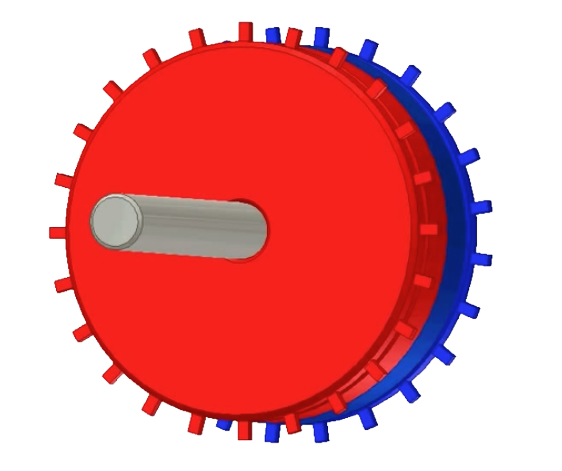
\includegraphics[scale=0.2]{images/hsm_operation/rotormag2}
		\caption{Rotor simplificado de um HSM (Com dentes)}
		\label{rotor2}
	\end{figure}
	
	O número de dentes também determina a resolução do passo: \emph{quanto mais dentes, menor a resolução}.
	
	De acordo com a Fig. \ref{rotor3}, verifica-se que os dentes de cada seção polar são espaçados com uma certa compensação devido a alinhação dos dentes. 
	
	\begin{figure}[!h]
		\centering 
		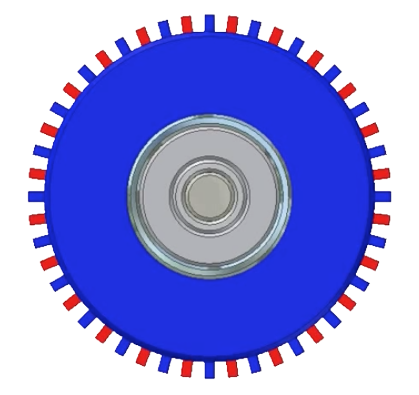
\includegraphics[scale=0.3]{images/hsm_operation/rotormag3}
		\caption{Visão superior do rotor de um HSM}
		\label{rotor3}
	\end{figure}
	
	Essa compensação funciona da seguinte forma: \emph{um dente de uma seção está sempre entre dois dentes da outra seção, alternando esta sequência}. Visualmente, temos a seguinte distribuição de dentes representada na Fig. \ref{rotor4}.
	
	\begin{figure}[!h]
		\centering 
		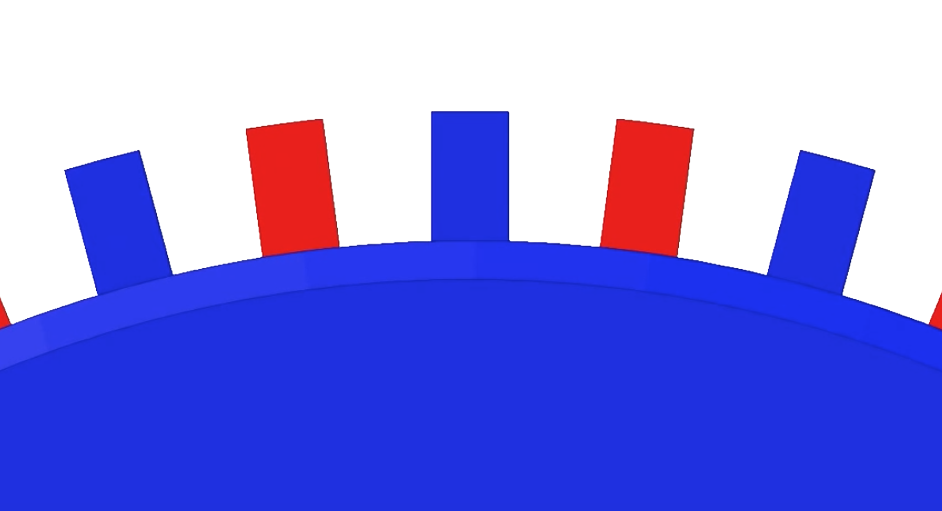
\includegraphics[scale=0.2]{images/hsm_operation/rotormag4}
		\caption{Visão superior do espaçamento entre os dentes das seções do rotor}
		\label{rotor4}
	\end{figure}
	
	Considerando um estator simples, com núcleo de metal, de duas fases com quatro enrolamentos, cada fase com dois enrolamentos (enrolamentos ligados em série), insere-se os enrolamentos na expressão gráfica apresentada anteriormente na Fig. \ref{rotor3}. O HSM simplificado para fins de explicação está representado na Fig \ref{hsm_superior}. 
	
	 \begin{figure}[!h]
		\centering 
		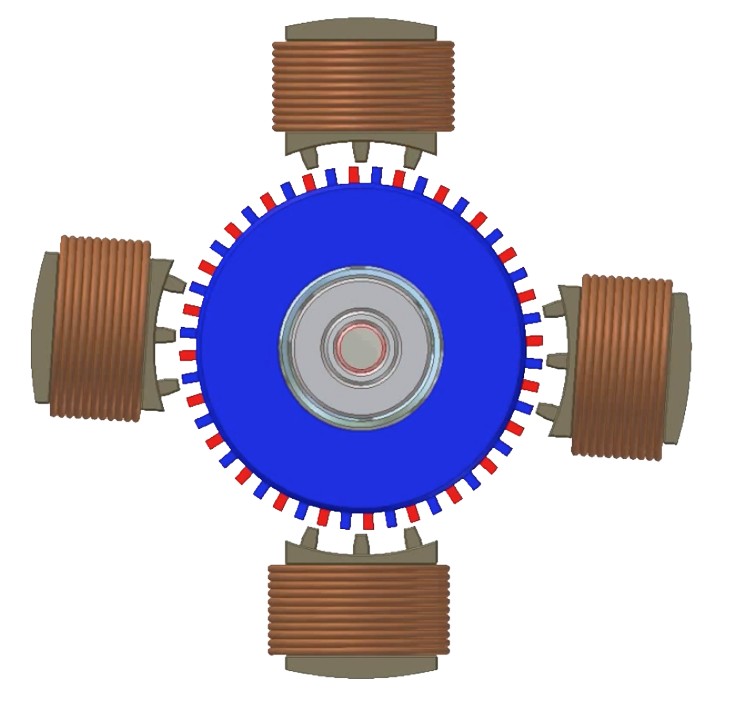
\includegraphics[scale=0.3]{images/hsm_operation/etapa1}
		\caption{Visão superior de um HSM, com estator e rotor em destaque}
		\label{hsm_superior}
	\end{figure}
	
	Com o estator e o rotor juntos, o princípio de funcionamento baseia-se em acionar uma das fases com um determinado sentido de corrente com o objetivo de magnetizar o núcleo metálico do estator.
	
	Em um dado momento, antes de acionar as bobinas de uma das fases, o estator se encontra em um estágio conforme a Fig. \ref{passo1}. 
	
	\begin{figure}[!h]
		\centering 
		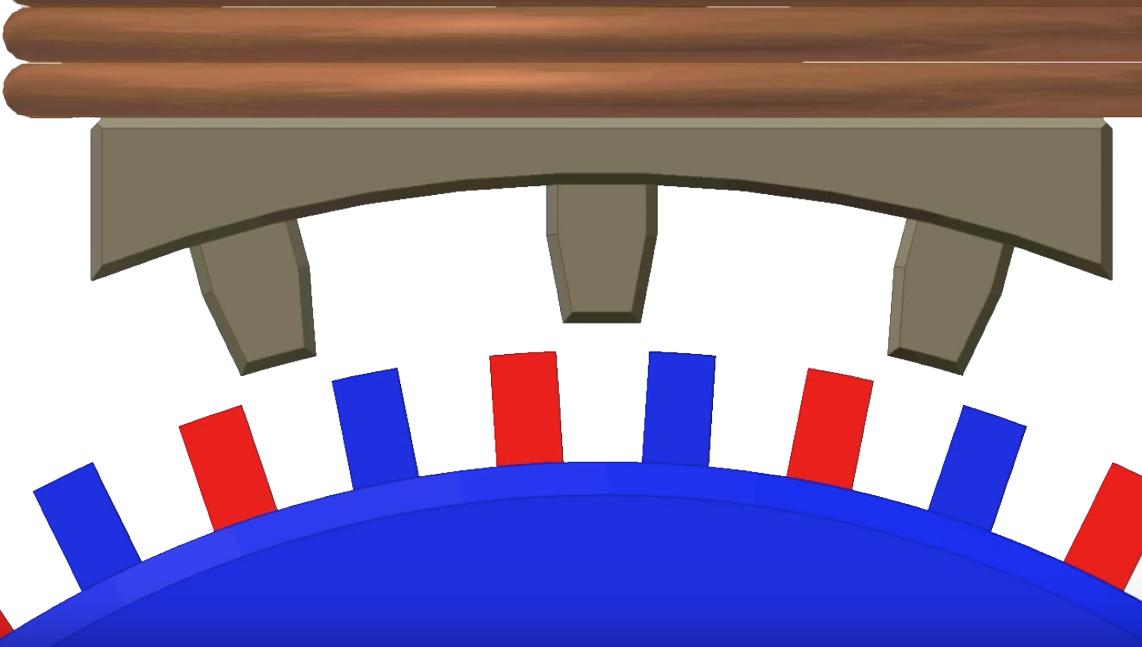
\includegraphics[scale=0.16]{images/hsm_operation/visaopasso1}
		\caption{Estator e rotor antes do acionamento das bobinas de uma fase}
		\label{passo1}
	\end{figure}
	
	Conforme a Fig. \ref{passo1}, assim que se aciona uma fase de forma com que a corrente nos enrolamentos crie um campo magnético no núcleo do estator, o estator se encontra com a seguinte polaridade magnética, conforme Fig. \ref{acionamento1}.
	
	\begin{figure}[!h]
		\centering 
		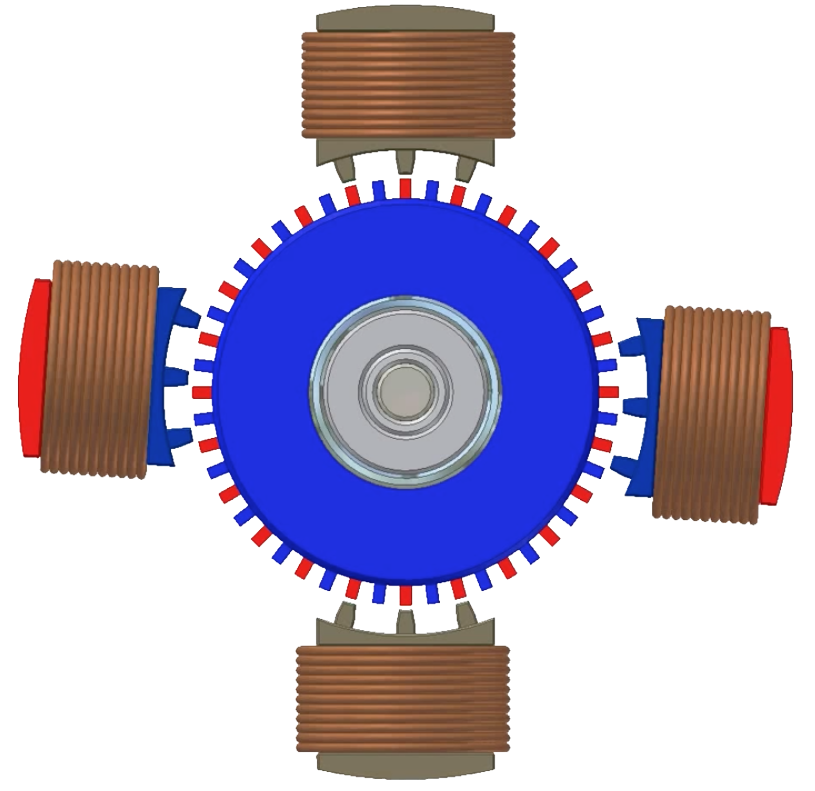
\includegraphics[scale=0.3]{images/hsm_operation/etapa3}
		\caption{Estator e rotor do HSM ao acionar uma das fases (núcleos do estator magnetizados horizontalmente)}
		\label{acionamento1}
	\end{figure}
	
	É importante relatar que os enrolamentos acionados estão em \textbf{série}, de forma com que o campo magnético direcionado para os dentes do rotor tenham a mesma polaridade, ou seja, o HSM analisado é \textbf{unipolar}. Essa característica de acionamento será melhor explanada na seção de Acionamentos do HSM.
	
	Com o núcleo do estator magnetizado como um eletroimã, em que a polaridade NORTE está direcionada ao rotor, tem-se a seguinte representação gráfica conforme a Fig. \ref{passo2}.
	
	\begin{figure}[!h]
		\centering 
		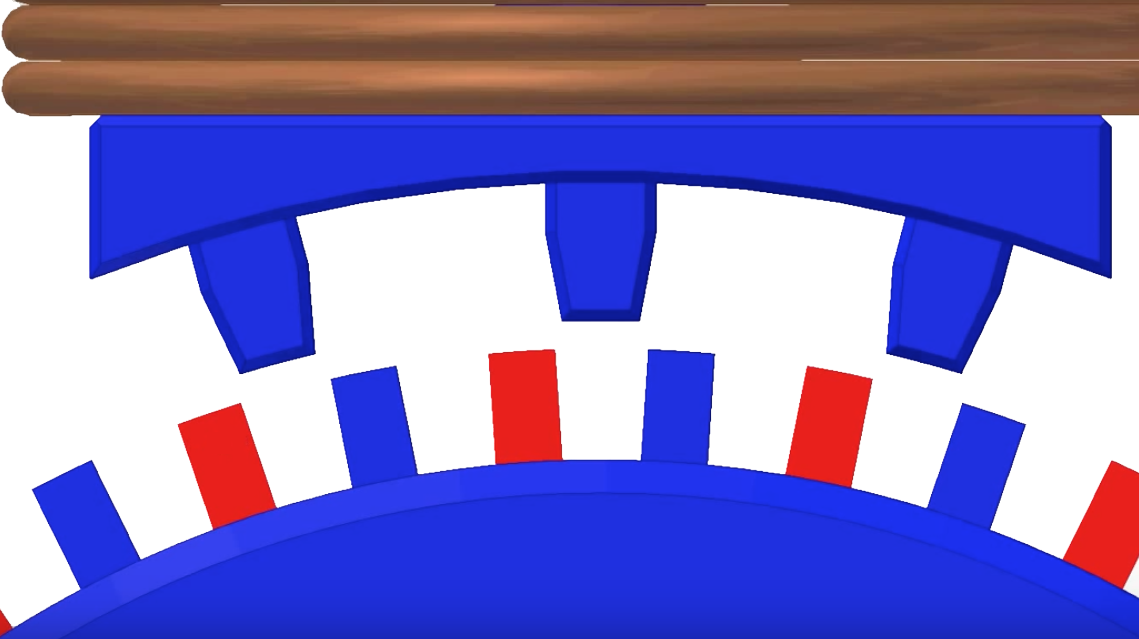
\includegraphics[scale=0.16]{images/hsm_operation/visaopasso2}
		\caption{Estator e rotor de um HSM ao acionar uma das fases}
		\label{passo2}
	\end{figure}
	
	Com isso, \textbf{ocorre uma atração magnética entre o dente da seção SUL do rotor e o dente do estator, polarizado como NORTE} e, de forma análoga, \textbf{ocorre uma repulsão magnética entre o dente da seção SUL do rotor e o dente do estator, polarizado como NORTE}.
	
	Esse movimento dos dentes do rotor devido a magnetização do núcleo do estator no motor de passo híbrido é a representação do \textbf{passo} do motor.
	
	A movimentação está indicada pelas setas na Fig. \ref{passo3}, conforme foi explanado.
	
	\begin{figure}[!h]
		\centering 
		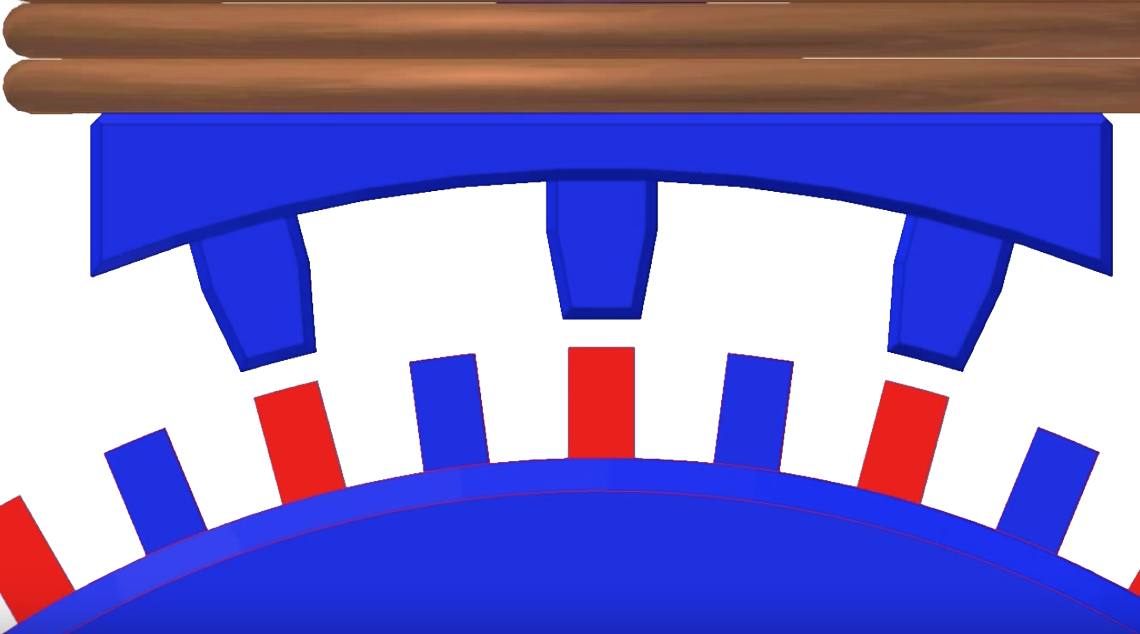
\includegraphics[scale=0.16]{images/hsm_operation/visaopasso3}
		\caption{Movimentação do rotor devido a magnetização do estator}
		\label{passo3}
	\end{figure}  
	
	Para efetuar mais um passo, basta acionar a outra fase do motor com o mesmo sentido de corrente, de forma com que seja magnetizado os núcleos de metal do estator pelo outro grupo de bobinas, conforme Fig. \ref{acionamento2}.
	
	\begin{figure}[!h]
		\centering 
		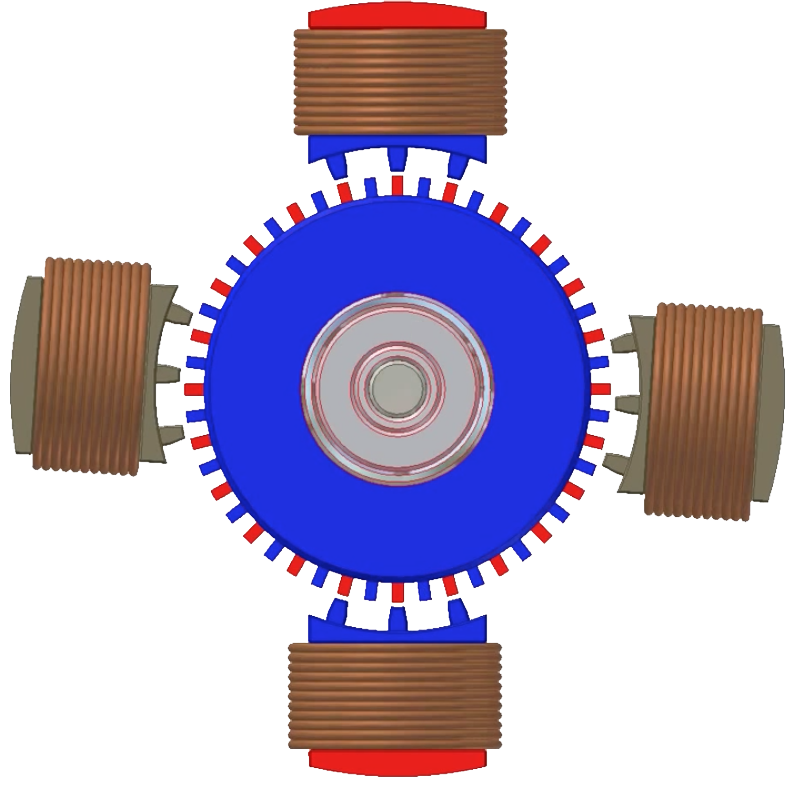
\includegraphics[scale=0.3]{images/hsm_operation/etapa2}
		\caption{Estator e rotor do HSM ao acionar outra fase (núcleos do estator magnetizados verticalmente)}
		\label{acionamento2}
	\end{figure}
	
	Repetindo o mesmo procedimento, o motor continuará executando os passos com a angulação determinada pela sequência e forma de acionamento das bobinas. Para \textbf{inverter o sentido de rotação do rotor}, basta inverter o sentido da corrente elétrica que flui pela fase, consequentemente pelos enrolamentos, e magnetizará o núcleo do estator que suporta os enrolamentos, como foi explanado durante toda esta seção do trabalho. 
	